%=====================================================================
\section{The two solution methods}
\label{sec:methods}

The same model is solved two ways. The MILP gives the \emph{exact} answer (and, where it finishes, a proof of
optimality); the reinforcement-learning (RL) policy gives a fast \emph{approximate} answer. Having both is what
lets every experiment be cross-checked: the two methods are independent, yet both are scored by the same checker,
so when they agree the number is trustworthy, and when only one of them can produce a plan that is informative too.

\subsection{Exact method: the MILP (Gurobi)}
The model of Section~\ref{sec:model} is handed to Gurobi unchanged --- the \emph{complete} formulation for every
instance size, with no reduction of the station, arc or neighbour sets. Each instance gets a warm start from a
fast greedy rule and a 300-second time limit; the run uses 8 instances in parallel $\times$ 4 threads (32 cores).
An instance ends \emph{optimal} (proven), \emph{time limit with a plan} (a feasible plan and a bound, hence a gap),
\emph{time limit with no plan}, or \emph{infeasible} (proven). The optimal instances are the gold standard the
rest of the report leans on, because on them the model's predictions can be checked exactly
(Section~\ref{sec:validation}).

\subsection{Learning method: an attention policy}
\textbf{The plan as a sequence of decisions.} Building a plan is a sequence of choices: pick an unserved EV, then
give it a gun or a van; repeat until all EVs are placed. This is a Markov decision process. The \emph{state}
holds which EVs are still unserved and the current load of every gun and van (earliest free time, remaining seats,
remaining battery). An \emph{action} picks an EV $i$ and a resource; a simulator then places the session as early
as feasible and updates the state. A \emph{mask} forbids any action that would break a constraint --- a station
out of range, a queue beyond $W_i$ \eqref{eq:qtol}, a finish after the deadline $T$ \eqref{eq:deadline}, a van
over seats \eqref{eq:vancap} or battery \eqref{eq:vanbatt} --- so every finished episode is a feasible plan (or
leaves an EV unplaceable, which marks the plan invalid, exactly as the MILP would be infeasible).

\textbf{The reward is the cost itself.} When an action places EV $i$, the reward is the increase in the objective
it causes, with a minus sign: $r_t=-\Delta Z_t$, where $\Delta Z_t$ is the sum of the terms of \eqref{eq:obj} that
the new session adds. This choice makes the learning objective \emph{identical} to the optimisation objective.

\begin{proposition}[the return is the negative plan cost]
\label{prop:return}
For any episode that places all EVs, the undiscounted return $G=\sum_t r_t$ equals $-Z$ of the plan it builds.
Hence a policy that maximises expected return minimises expected $Z$.
\end{proposition}
\begin{proof}
The objective \eqref{eq:obj} is a sum over EVs (and van arcs, each introduced with its EV) of non-negative terms.
Placing EV $i$ adds exactly its terms $\Delta Z_t$ to $Z$, and every term of $Z$ is added by exactly one placement,
so $\sum_t \Delta Z_t=Z$ (a telescoping sum over a partition of the objective's terms). Therefore
$G=\sum_t(-\Delta Z_t)=-Z$. Maximising $\mathbb E[G]=-\mathbb E[Z]$ minimises $\mathbb E[Z]$.
\end{proof}

A second fact justifies the simulator placing each session as early as possible.
\begin{proposition}[earliest start is optimal for a fixed order]
\label{prop:earliest}
Given the assignment of every EV to a resource and the order in which a gun or van serves its EVs, scheduling each
session at its earliest feasible start minimises every time term in $Z_6$ and never tightens the deadline
\eqref{eq:deadline}.
\end{proposition}
\begin{proof}
In $Z_6$ the queue $q^{\mathrm F}_i$, the van wait $q^{\mathrm M}_i$ and the completion $C_i=S_i+\tau$ are all
non-decreasing in the start $S_i$; the charging and drive durations are fixed by \eqref{eq:tau}. Delaying any $S_i$
can only raise these terms and move $C_i$ towards the deadline, never the reverse. So the earliest feasible start
is optimal term by term, and feasibility of a later start implies feasibility of the earliest one.
\end{proof}

\textbf{The network.} Figure~\ref{fig:rl} shows the policy. An \emph{encoder} (multi-head attention, after
Kool et al.\ 2019) reads every EV, station and van with its features --- position, energy, request time, and the
\emph{segment and income} $(s_i,\theta_i)$ and the coefficients they imply --- and produces an embedding for each.
A \emph{two-step decoder} (after Li et al.\ 2021) then, at each step, attends over the embeddings to pick the next
EV and then its resource (a gun or a van), subject to the mask. The policy is trained with REINFORCE using a
\emph{POMO} shared baseline: several rollouts of the same instance from different first moves share a baseline, so
the gradient rewards a rollout only for beating its siblings, which lowers variance without a learned critic.

\begin{figure}[H]
\centering
\begin{tikzpicture}[font=\footnotesize,>={Stealth[length=2mm]},
  b/.style={draw,rounded corners,align=center,minimum height=0.95cm,inner sep=4pt},node distance=4mm]
  \node[b,fill=accent!12] (inst) {instance\\ EVs, FCS, vans\\ $(s_i,\theta_i)$};
  \node[b,fill=headblue!10,right=7mm of inst] (enc) {attention\\ encoder};
  \node[b,fill=accent3!12,right=7mm of enc] (dec) {two-step decoder\\ pick EV $\to$ gun/van};
  \node[b,fill=orange!10,right=7mm of dec] (sim) {simulator\\ earliest start,\\ masks};
  \node[b,fill=accent2!12,right=7mm of sim] (rew) {plan\\ reward $-\Delta Z$};
  \draw[->] (inst)--(enc); \draw[->] (enc)--(dec); \draw[->] (dec)--(sim); \draw[->] (sim)--(rew);
  \draw[->] (sim.south) to[out=-90,in=-90] node[below,font=\scriptsize]{until all EVs placed} (dec.south);
\end{tikzpicture}
\caption{The RL policy. The encoder embeds every EV, station and van (including segment and income); the decoder
places EVs one at a time; the simulator schedules each at its earliest feasible time and masks infeasible moves;
the reward is $-\Delta Z$, so the return is $-Z$ (Proposition~\ref{prop:return}).}
\label{fig:rl}
\end{figure}

\textbf{Training.} A generator draws random instances in the style of the data. Each model trains for a
\emph{minimum} of 200 epochs (early stopping is disabled until then), then stops after 10 epochs without a better
validation score, at 500 epochs, or an 8-hour cap --- whichever comes first (Figure~\ref{fig:training}). For an
experiment variant the policy is \emph{retrained} on instances carrying that variant's change, so it is
re-optimised for the new setting, not merely re-applied.

\begin{figure}[H]
\centering
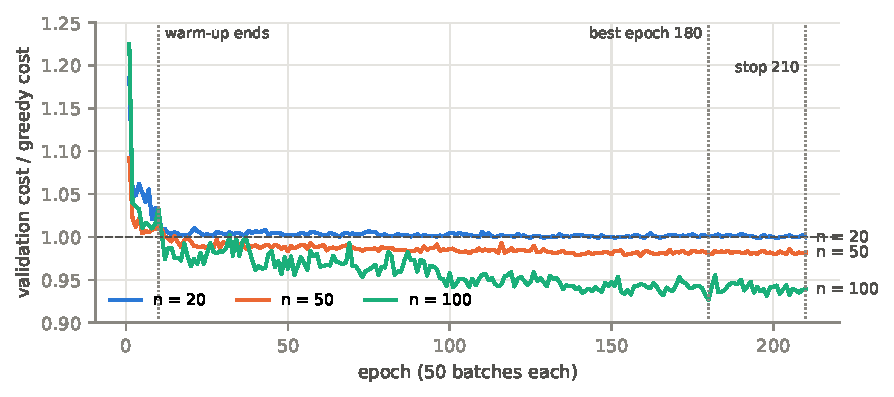
\includegraphics[width=0.86\textwidth]{figures/rl_training.pdf}
\caption{Baseline training: validation cost relative to the greedy rule, by instance size, over epochs
($\frlParams$ parameters, best at epoch \frlBestEpoch).}
\label{fig:training}
\end{figure}

\subsection{Why the two methods are comparable}
Every plan --- from Gurobi, from the greedy rule or from the RL policy --- is written in the same format and scored
by \emph{one} independent checker that re-tests constraints (2)--(23) and recomputes the objective \eqref{eq:obj}.
Neither method is trusted to report its own cost. So a cost difference between the MILP and RL is a real difference
in plan quality, and the $Z$ change an experiment produces can be read off either method and compared
(Section~\ref{sec:milpvsrl}). This shared, neutral yardstick is the backbone of the ``support'' step in every
result below.

\inshort{Gurobi solves the exact model; an attention policy trained with REINFORCE$+$POMO solves it fast, with the
reward set so that maximising return is exactly minimising $Z$ (Proposition~\ref{prop:return}). A single
independent checker scores both, which is what makes the two methods a cross-check on each other.}
